% Options for packages loaded elsewhere
\PassOptionsToPackage{unicode}{hyperref}
\PassOptionsToPackage{hyphens}{url}
\PassOptionsToPackage{dvipsnames,svgnames,x11names}{xcolor}
%
\documentclass[
  letterpaper,
  DIV=11,
  numbers=noendperiod]{scrartcl}

\usepackage{amsmath,amssymb}
\usepackage{iftex}
\ifPDFTeX
  \usepackage[T1]{fontenc}
  \usepackage[utf8]{inputenc}
  \usepackage{textcomp} % provide euro and other symbols
\else % if luatex or xetex
  \usepackage{unicode-math}
  \defaultfontfeatures{Scale=MatchLowercase}
  \defaultfontfeatures[\rmfamily]{Ligatures=TeX,Scale=1}
\fi
\usepackage{lmodern}
\ifPDFTeX\else  
    % xetex/luatex font selection
\fi
% Use upquote if available, for straight quotes in verbatim environments
\IfFileExists{upquote.sty}{\usepackage{upquote}}{}
\IfFileExists{microtype.sty}{% use microtype if available
  \usepackage[]{microtype}
  \UseMicrotypeSet[protrusion]{basicmath} % disable protrusion for tt fonts
}{}
\makeatletter
\@ifundefined{KOMAClassName}{% if non-KOMA class
  \IfFileExists{parskip.sty}{%
    \usepackage{parskip}
  }{% else
    \setlength{\parindent}{0pt}
    \setlength{\parskip}{6pt plus 2pt minus 1pt}}
}{% if KOMA class
  \KOMAoptions{parskip=half}}
\makeatother
\usepackage{xcolor}
\setlength{\emergencystretch}{3em} % prevent overfull lines
\setcounter{secnumdepth}{-\maxdimen} % remove section numbering
% Make \paragraph and \subparagraph free-standing
\makeatletter
\ifx\paragraph\undefined\else
  \let\oldparagraph\paragraph
  \renewcommand{\paragraph}{
    \@ifstar
      \xxxParagraphStar
      \xxxParagraphNoStar
  }
  \newcommand{\xxxParagraphStar}[1]{\oldparagraph*{#1}\mbox{}}
  \newcommand{\xxxParagraphNoStar}[1]{\oldparagraph{#1}\mbox{}}
\fi
\ifx\subparagraph\undefined\else
  \let\oldsubparagraph\subparagraph
  \renewcommand{\subparagraph}{
    \@ifstar
      \xxxSubParagraphStar
      \xxxSubParagraphNoStar
  }
  \newcommand{\xxxSubParagraphStar}[1]{\oldsubparagraph*{#1}\mbox{}}
  \newcommand{\xxxSubParagraphNoStar}[1]{\oldsubparagraph{#1}\mbox{}}
\fi
\makeatother

\usepackage{color}
\usepackage{fancyvrb}
\newcommand{\VerbBar}{|}
\newcommand{\VERB}{\Verb[commandchars=\\\{\}]}
\DefineVerbatimEnvironment{Highlighting}{Verbatim}{commandchars=\\\{\}}
% Add ',fontsize=\small' for more characters per line
\usepackage{framed}
\definecolor{shadecolor}{RGB}{241,243,245}
\newenvironment{Shaded}{\begin{snugshade}}{\end{snugshade}}
\newcommand{\AlertTok}[1]{\textcolor[rgb]{0.68,0.00,0.00}{#1}}
\newcommand{\AnnotationTok}[1]{\textcolor[rgb]{0.37,0.37,0.37}{#1}}
\newcommand{\AttributeTok}[1]{\textcolor[rgb]{0.40,0.45,0.13}{#1}}
\newcommand{\BaseNTok}[1]{\textcolor[rgb]{0.68,0.00,0.00}{#1}}
\newcommand{\BuiltInTok}[1]{\textcolor[rgb]{0.00,0.23,0.31}{#1}}
\newcommand{\CharTok}[1]{\textcolor[rgb]{0.13,0.47,0.30}{#1}}
\newcommand{\CommentTok}[1]{\textcolor[rgb]{0.37,0.37,0.37}{#1}}
\newcommand{\CommentVarTok}[1]{\textcolor[rgb]{0.37,0.37,0.37}{\textit{#1}}}
\newcommand{\ConstantTok}[1]{\textcolor[rgb]{0.56,0.35,0.01}{#1}}
\newcommand{\ControlFlowTok}[1]{\textcolor[rgb]{0.00,0.23,0.31}{\textbf{#1}}}
\newcommand{\DataTypeTok}[1]{\textcolor[rgb]{0.68,0.00,0.00}{#1}}
\newcommand{\DecValTok}[1]{\textcolor[rgb]{0.68,0.00,0.00}{#1}}
\newcommand{\DocumentationTok}[1]{\textcolor[rgb]{0.37,0.37,0.37}{\textit{#1}}}
\newcommand{\ErrorTok}[1]{\textcolor[rgb]{0.68,0.00,0.00}{#1}}
\newcommand{\ExtensionTok}[1]{\textcolor[rgb]{0.00,0.23,0.31}{#1}}
\newcommand{\FloatTok}[1]{\textcolor[rgb]{0.68,0.00,0.00}{#1}}
\newcommand{\FunctionTok}[1]{\textcolor[rgb]{0.28,0.35,0.67}{#1}}
\newcommand{\ImportTok}[1]{\textcolor[rgb]{0.00,0.46,0.62}{#1}}
\newcommand{\InformationTok}[1]{\textcolor[rgb]{0.37,0.37,0.37}{#1}}
\newcommand{\KeywordTok}[1]{\textcolor[rgb]{0.00,0.23,0.31}{\textbf{#1}}}
\newcommand{\NormalTok}[1]{\textcolor[rgb]{0.00,0.23,0.31}{#1}}
\newcommand{\OperatorTok}[1]{\textcolor[rgb]{0.37,0.37,0.37}{#1}}
\newcommand{\OtherTok}[1]{\textcolor[rgb]{0.00,0.23,0.31}{#1}}
\newcommand{\PreprocessorTok}[1]{\textcolor[rgb]{0.68,0.00,0.00}{#1}}
\newcommand{\RegionMarkerTok}[1]{\textcolor[rgb]{0.00,0.23,0.31}{#1}}
\newcommand{\SpecialCharTok}[1]{\textcolor[rgb]{0.37,0.37,0.37}{#1}}
\newcommand{\SpecialStringTok}[1]{\textcolor[rgb]{0.13,0.47,0.30}{#1}}
\newcommand{\StringTok}[1]{\textcolor[rgb]{0.13,0.47,0.30}{#1}}
\newcommand{\VariableTok}[1]{\textcolor[rgb]{0.07,0.07,0.07}{#1}}
\newcommand{\VerbatimStringTok}[1]{\textcolor[rgb]{0.13,0.47,0.30}{#1}}
\newcommand{\WarningTok}[1]{\textcolor[rgb]{0.37,0.37,0.37}{\textit{#1}}}

\providecommand{\tightlist}{%
  \setlength{\itemsep}{0pt}\setlength{\parskip}{0pt}}\usepackage{longtable,booktabs,array}
\usepackage{calc} % for calculating minipage widths
% Correct order of tables after \paragraph or \subparagraph
\usepackage{etoolbox}
\makeatletter
\patchcmd\longtable{\par}{\if@noskipsec\mbox{}\fi\par}{}{}
\makeatother
% Allow footnotes in longtable head/foot
\IfFileExists{footnotehyper.sty}{\usepackage{footnotehyper}}{\usepackage{footnote}}
\makesavenoteenv{longtable}
\usepackage{graphicx}
\makeatletter
\newsavebox\pandoc@box
\newcommand*\pandocbounded[1]{% scales image to fit in text height/width
  \sbox\pandoc@box{#1}%
  \Gscale@div\@tempa{\textheight}{\dimexpr\ht\pandoc@box+\dp\pandoc@box\relax}%
  \Gscale@div\@tempb{\linewidth}{\wd\pandoc@box}%
  \ifdim\@tempb\p@<\@tempa\p@\let\@tempa\@tempb\fi% select the smaller of both
  \ifdim\@tempa\p@<\p@\scalebox{\@tempa}{\usebox\pandoc@box}%
  \else\usebox{\pandoc@box}%
  \fi%
}
% Set default figure placement to htbp
\def\fps@figure{htbp}
\makeatother

\usepackage{booktabs}
\usepackage{longtable}
\usepackage{array}
\usepackage{multirow}
\usepackage{wrapfig}
\usepackage{float}
\usepackage{colortbl}
\usepackage{pdflscape}
\usepackage{tabu}
\usepackage{threeparttable}
\usepackage{threeparttablex}
\usepackage[normalem]{ulem}
\usepackage{makecell}
\usepackage{xcolor}
\KOMAoption{captions}{tableheading}
\makeatletter
\@ifpackageloaded{caption}{}{\usepackage{caption}}
\AtBeginDocument{%
\ifdefined\contentsname
  \renewcommand*\contentsname{Table of contents}
\else
  \newcommand\contentsname{Table of contents}
\fi
\ifdefined\listfigurename
  \renewcommand*\listfigurename{List of Figures}
\else
  \newcommand\listfigurename{List of Figures}
\fi
\ifdefined\listtablename
  \renewcommand*\listtablename{List of Tables}
\else
  \newcommand\listtablename{List of Tables}
\fi
\ifdefined\figurename
  \renewcommand*\figurename{Figure}
\else
  \newcommand\figurename{Figure}
\fi
\ifdefined\tablename
  \renewcommand*\tablename{Table}
\else
  \newcommand\tablename{Table}
\fi
}
\@ifpackageloaded{float}{}{\usepackage{float}}
\floatstyle{ruled}
\@ifundefined{c@chapter}{\newfloat{codelisting}{h}{lop}}{\newfloat{codelisting}{h}{lop}[chapter]}
\floatname{codelisting}{Listing}
\newcommand*\listoflistings{\listof{codelisting}{List of Listings}}
\makeatother
\makeatletter
\makeatother
\makeatletter
\@ifpackageloaded{caption}{}{\usepackage{caption}}
\@ifpackageloaded{subcaption}{}{\usepackage{subcaption}}
\makeatother

\usepackage{bookmark}

\IfFileExists{xurl.sty}{\usepackage{xurl}}{} % add URL line breaks if available
\urlstyle{same} % disable monospaced font for URLs
\hypersetup{
  pdftitle={Assignment 1 --- MSB104 --- Group 3},
  pdfauthor={Irjan \& Magnus},
  colorlinks=true,
  linkcolor={blue},
  filecolor={Maroon},
  citecolor={Blue},
  urlcolor={Blue},
  pdfcreator={LaTeX via pandoc}}


\title{Assignment 1 --- MSB104 --- Group 3}
\author{Irjan \& Magnus}
\date{}

\begin{document}
\maketitle


\section{Part A Sub-national GDP and GDP per
capita}\label{part-a-sub-national-gdp-and-gdp-per-capita}

\subsection{Data aquisition}\label{data-aquisition}

\begin{Shaded}
\begin{Highlighting}[]
\CommentTok{\# Henter inn populasjons datasett fra excell}
\NormalTok{Populasjon }\OtherTok{\textless{}{-}} \FunctionTok{read\_excel}\NormalTok{(}\StringTok{"DEMO\_Ass1.xlsx"}\NormalTok{, }\AttributeTok{sheet =} \DecValTok{2}\NormalTok{, }\AttributeTok{col\_types =} \StringTok{"text"}\NormalTok{) }\SpecialCharTok{\%\textgreater{}\%}
  \FunctionTok{clean\_names}\NormalTok{()}

\CommentTok{\# Henter inn regional BNP datasett fra excell}
\NormalTok{BNP }\OtherTok{\textless{}{-}} \FunctionTok{read\_excel}\NormalTok{(}\StringTok{"GDP\_Ass1.xlsx"}\NormalTok{, }\AttributeTok{sheet =} \DecValTok{2}\NormalTok{, }\AttributeTok{col\_types =} \StringTok{"text"}\NormalTok{) }\SpecialCharTok{\%\textgreater{}\%}
  \FunctionTok{clean\_names}\NormalTok{()}
\end{Highlighting}
\end{Shaded}

\begin{Shaded}
\begin{Highlighting}[]
\CommentTok{\# Omgjør Populasjonen til langt format}

\NormalTok{PopulasjonLang }\OtherTok{\textless{}{-}}\NormalTok{ Populasjon }\SpecialCharTok{\%\textgreater{}\%}
  \FunctionTok{pivot\_longer}\NormalTok{(}
    \AttributeTok{cols =} \FunctionTok{starts\_with}\NormalTok{(}\StringTok{"x"}\NormalTok{),}
    \AttributeTok{names\_to =} \StringTok{"aar"}\NormalTok{,}
    \AttributeTok{values\_to =} \StringTok{"befolkning"}
\NormalTok{  ) }\SpecialCharTok{\%\textgreater{}\%}
  \FunctionTok{mutate}\NormalTok{(}
    \AttributeTok{aar =} \FunctionTok{as.integer}\NormalTok{(}\FunctionTok{str\_remove}\NormalTok{(aar, }\StringTok{"\^{}x"}\NormalTok{)),}
    \AttributeTok{befolkning =} \FunctionTok{as.numeric}\NormalTok{(}\FunctionTok{str\_replace\_all}\NormalTok{(befolkning, }\StringTok{" "}\NormalTok{, }\StringTok{""}\NormalTok{))}
\NormalTok{  )}

\CommentTok{\# Omgjør BNP til langt format}

\NormalTok{BNPLang }\OtherTok{\textless{}{-}}\NormalTok{ BNP }\SpecialCharTok{\%\textgreater{}\%}
  \FunctionTok{pivot\_longer}\NormalTok{(}
    \AttributeTok{cols =} \FunctionTok{starts\_with}\NormalTok{(}\StringTok{"x"}\NormalTok{),}
    \AttributeTok{names\_to =} \StringTok{"aar"}\NormalTok{,}
    \AttributeTok{values\_to =} \StringTok{"BNP"}
\NormalTok{  ) }\SpecialCharTok{\%\textgreater{}\%}
  \FunctionTok{mutate}\NormalTok{(}
    \AttributeTok{aar =} \FunctionTok{as.integer}\NormalTok{(}\FunctionTok{str\_remove}\NormalTok{(aar, }\StringTok{"\^{}x"}\NormalTok{)),}
    \AttributeTok{BNP =} \FunctionTok{as.numeric}\NormalTok{(}\FunctionTok{str\_replace\_all}\NormalTok{(BNP, }\StringTok{" "}\NormalTok{, }\StringTok{""}\NormalTok{))}
\NormalTok{  )}
\end{Highlighting}
\end{Shaded}

\subsubsection{Kort gjennomgang av datasett og
variabler}\label{kort-gjennomgang-av-datasett-og-variabler}

Datasette \emph{demo\_r\_pjanggr3} som er hentet fra Eurostat inneholder
årlige befolkningestimater på NUTS3-nivå for EU-, EFTA- og kandidatland.
Variablene \textbf{values} viser totalt antall bosatte personer per 1.
januar, målt i antall personer. Hver observasjon identifiseres ved
regionkode(\textbf{geo}) og år (\textbf{time}), samnt kjønn
(\textbf{sex}) og alder (\textbf{age}). I denne analysen benyttes kun
total befolkning (\textbf{sex = T},\textbf{age = TOTAL}), slik at
dataene ikke er splittet etter kjønn eller alder.

Det finnes ulike hoved metoder å beregne brytto nasjonalt produkt på.
Eurostat har valgt å benytte den såkalte «inntekstmetoden». Eurostat
velger denne metoden ovenfor utgifts metoden grunnet mangel på data over
gode overføringer mellom regioner.

Etter inntektsmetoden regnes BNP på følgende måte: Lønn som utbetales
til ansatte + bedrifter sin fortjeneste + skatte og avgifter minus
subsidier gitt fra staten + avskrivinger knyttet til industri.

\subsection{BNP per innbygger}\label{bnp-per-innbygger}

\begin{Shaded}
\begin{Highlighting}[]
\CommentTok{\# Kombinerer tabellene og filtrerer bort NA{-}verdiene}


\NormalTok{KombinertRen }\OtherTok{\textless{}{-}}\NormalTok{ Kombinert }\SpecialCharTok{\%\textgreater{}\%}
  \FunctionTok{filter}\NormalTok{(}\SpecialCharTok{!}\FunctionTok{is.na}\NormalTok{(BNPPI))}
\end{Highlighting}
\end{Shaded}

\begin{verbatim}
[1] 4680
\end{verbatim}

\begin{verbatim}
# A tibble: 1 x 6
    geo region   aar befolkning   BNP BNPPI
  <int>  <int> <int>      <int> <int> <int>
1     0      0     0        358   515   841
\end{verbatim}

I tabellene over har vi kombinert de to datasettene hentet fra Eurostat.
Vi har da en tabell som viser BNP per innbygger i hvert av NUTS3
områdene for delt på år. I hver observasjon hvor det forekommer en NA
verdi i populasjon og eller total BNP vil også få BNPPI som NA verdi.
Datasettet består av totalt 4680 observasjoner, og 841 av dem ender opp
ned NA verdi i BNPPI. For å videre kunne jobbe mer effektivt i
utarbeidelsen av tabellene, lager vi et nytt datasett hvor alle
observasjoner med NA verdi er fjernet.

\begin{longtable}[]{@{}crrrr@{}}
\caption{Utvikling i BNP per innbygger (gjennomsnitt, median, minimum og
maksimum) per år}\tabularnewline
\toprule\noalign{}
År & Gjennomsnitt BNPPI & Median BNPPI & Minste BNPPI & Største BNPPI \\
\midrule\noalign{}
\endfirsthead
\toprule\noalign{}
År & Gjennomsnitt BNPPI & Median BNPPI & Minste BNPPI & Største BNPPI \\
\midrule\noalign{}
\endhead
\bottomrule\noalign{}
\endlastfoot
2000 & 7 332 & 1 693 & 825 & 36 461 \\
2001 & 15 681 & 17 764 & 1 025 & 38 652 \\
2002 & 16 259 & 17 984 & 1 066 & 40 238 \\
2003 & 16 783 & 18 392 & 1 235 & 41 704 \\
2004 & 17 440 & 19 381 & 1 338 & 43 010 \\
2005 & 17 965 & 19 786 & 1 534 & 44 057 \\
2006 & 18 864 & 20 647 & 1 998 & 44 605 \\
2007 & 19 915 & 21 431 & 2 460 & 47 618 \\
2008 & 20 082 & 20 872 & 3 142 & 50 967 \\
2009 & 18 903 & 20 146 & 2 583 & 49 307 \\
2010 & 19 251 & 20 559 & 2 606 & 52 021 \\
2011 & 19 842 & 21 112 & 2 760 & 52 664 \\
2012 & 19 786 & 20 939 & 3 074 & 51 194 \\
2013 & 19 713 & 20 422 & 3 381 & 50 043 \\
2014 & 19 952 & 20 254 & 3 507 & 50 629 \\
2015 & 20 357 & 20 710 & 3 663 & 51 592 \\
2016 & 20 832 & 21 068 & 3 833 & 53 373 \\
2017 & 21 655 & 21 609 & 4 349 & 54 406 \\
2018 & 22 323 & 22 850 & 4 982 & 55 923 \\
2019 & 22 879 & 23 372 & 5 274 & 57 074 \\
2020 & 21 605 & 21 358 & 5 250 & 55 637 \\
2021 & 23 863 & 23 849 & 5 685 & 61 275 \\
2022 & 26 170 & 25 664 & 6 070 & 66 633 \\
2023 & 22 906 & 15 014 & 6 989 & 61 545 \\
\end{longtable}

I tabellen over ser vi utviklingen av gjennomsnitt, median, minste og
høyeste verdi for BNP per inbygger for fra år 2000 til år 2023. Verdiene
er basert på alle observasjonene fra datasettet hvor observasjoner med
NA verdier er fjernet. Videre skal vi lage en deskriptiv analyse utifra
statistikken som fremkommer av datasettet. For å enklere visualisere
dette lager vi linediagrammer for sentrale mål.

\pandocbounded{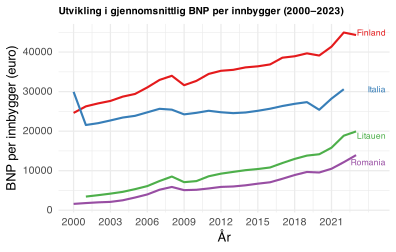
\includegraphics[keepaspectratio]{Assignment1_MSB104_files/figure-pdf/unnamed-chunk-10-1.pdf}}

\begin{verbatim}
[1] "geo"        "region"     "aar"        "befolkning" "BNP"       
[6] "BNPPI"     
\end{verbatim}

\begin{Shaded}
\begin{Highlighting}[]
\CommentTok{\# 1. Beregn gjennomsnitt per land og år}
\NormalTok{KombinertRen }\OtherTok{\textless{}{-}}\NormalTok{ KombinertRen }\SpecialCharTok{\%\textgreater{}\%}
  \FunctionTok{mutate}\NormalTok{(}
    \AttributeTok{land =} \FunctionTok{substr}\NormalTok{( geo, }\DecValTok{1}\NormalTok{, }\DecValTok{2}\NormalTok{)}
\NormalTok{  )}
\NormalTok{SnittTidLand }\OtherTok{\textless{}{-}}\NormalTok{ KombinertRen }\SpecialCharTok{\%\textgreater{}\%}
  \FunctionTok{group\_by}\NormalTok{(land, aar) }\SpecialCharTok{\%\textgreater{}\%}
  \FunctionTok{summarise}\NormalTok{(}
    \AttributeTok{gjennomsnitt\_bnp =} \FunctionTok{mean}\NormalTok{(BNPPI, }\AttributeTok{na.rm =} \ConstantTok{TRUE}\NormalTok{),}
    \AttributeTok{.groups =} \StringTok{"drop"}
\NormalTok{  )}

\CommentTok{\# 2. Bytt ut landkodene med fulle navn}
\NormalTok{SnittTidLand }\OtherTok{\textless{}{-}}\NormalTok{ SnittTidLand }\SpecialCharTok{\%\textgreater{}\%}
  \FunctionTok{mutate}\NormalTok{(}
    \AttributeTok{land\_navn =} \FunctionTok{recode}\NormalTok{(land,}
      \StringTok{"IT"} \OtherTok{=} \StringTok{"Italia"}\NormalTok{,}
      \StringTok{"FI"} \OtherTok{=} \StringTok{"Finland"}\NormalTok{,}
      \StringTok{"LT"} \OtherTok{=} \StringTok{"Litauen"}\NormalTok{,}
      \StringTok{"RO"} \OtherTok{=} \StringTok{"Romania"}
\NormalTok{    )}
\NormalTok{  )}

\CommentTok{\# 3. Finn siste observasjon for etikettplassering}
\NormalTok{etiketter }\OtherTok{\textless{}{-}}\NormalTok{ SnittTidLand }\SpecialCharTok{\%\textgreater{}\%}
  \FunctionTok{group\_by}\NormalTok{(land\_navn) }\SpecialCharTok{\%\textgreater{}\%}
  \FunctionTok{filter}\NormalTok{(aar }\SpecialCharTok{==} \FunctionTok{max}\NormalTok{(aar))}

\CommentTok{\# 4. Lag linjediagram med etiketter}
\FunctionTok{ggplot}\NormalTok{(SnittTidLand, }\FunctionTok{aes}\NormalTok{(}\AttributeTok{x =}\NormalTok{ aar, }\AttributeTok{y =}\NormalTok{ gjennomsnitt\_bnp, }\AttributeTok{color =}\NormalTok{ land\_navn)) }\SpecialCharTok{+}
  \FunctionTok{geom\_line}\NormalTok{(}\AttributeTok{linewidth =} \DecValTok{1}\NormalTok{) }\SpecialCharTok{+}
  \FunctionTok{geom\_point}\NormalTok{(}\AttributeTok{size =} \DecValTok{2}\NormalTok{) }\SpecialCharTok{+}
  \FunctionTok{geom\_text\_repel}\NormalTok{(}
    \AttributeTok{data =}\NormalTok{ etiketter,}
    \FunctionTok{aes}\NormalTok{(}\AttributeTok{label =}\NormalTok{ land\_navn),}
    \AttributeTok{nudge\_x =} \FloatTok{2.5}\NormalTok{,}
    \AttributeTok{size =} \DecValTok{3}\NormalTok{,}
    \AttributeTok{direction =} \StringTok{"y"}\NormalTok{,}
    \AttributeTok{hjust =} \DecValTok{0}\NormalTok{,}
    \AttributeTok{segment.color =} \ConstantTok{NA}
\NormalTok{  ) }\SpecialCharTok{+}
  \FunctionTok{scale\_x\_continuous}\NormalTok{(}
    \AttributeTok{breaks =} \FunctionTok{seq}\NormalTok{(}\DecValTok{2000}\NormalTok{, }\DecValTok{2023}\NormalTok{, }\DecValTok{3}\NormalTok{)}
\NormalTok{  ) }\SpecialCharTok{+}
  \FunctionTok{scale\_color\_brewer}\NormalTok{(}\AttributeTok{palette =} \StringTok{"Set1"}\NormalTok{) }\SpecialCharTok{+}
  \FunctionTok{labs}\NormalTok{(}
    \AttributeTok{title =} \StringTok{"Utvikling i gjennomsnittlig BNP per innbygger (2000–2023)"}\NormalTok{,}
    \AttributeTok{x =} \StringTok{"År"}\NormalTok{,}
    \AttributeTok{y =} \StringTok{"BNP per innbygger (euro)"}\NormalTok{,}
    \AttributeTok{color =} \ConstantTok{NULL}
\NormalTok{  ) }\SpecialCharTok{+}
  \FunctionTok{theme\_minimal}\NormalTok{(}\AttributeTok{base\_size =} \DecValTok{13}\NormalTok{) }\SpecialCharTok{+}
  \FunctionTok{theme}\NormalTok{(}
    \AttributeTok{plot.title =} \FunctionTok{element\_text}\NormalTok{(}\AttributeTok{face =} \StringTok{"bold"}\NormalTok{, }\AttributeTok{size =} \DecValTok{10}\NormalTok{),}
    \AttributeTok{legend.position =} \StringTok{"none"}\NormalTok{,}
\NormalTok{  )}
\end{Highlighting}
\end{Shaded}

\pandocbounded{\includegraphics[keepaspectratio]{Assignment1_MSB104_files/figure-pdf/unnamed-chunk-12-1.pdf}}

I tabellene over ser vi utviklingen av gjennomsnitt og median verdien
fra år 2000 til 2023. Begge de statistiske målene følger i stor grad
samme utvikling. Det er en stor økning fra 2000 til 2001. Etter dette er
det i hovedsak en jevn generelt vekst fra år til år, med et par avvik. I
både 2008 og 2020 ser vi reduksjon i BNPPI sammenlignet med det
forekommende året. I 2023 ser vi igjen en drastisk endring, spesielt i
Median hvor BNPPI reduseres fra ca 25 000 dollar til ca 15 000 dollar.
Reduksjonen i år 2008 og 2020 er ikke overraskende og kan forklares med
henholdsvis finanskrisen og Covid-19.

En annen faktor som kan påvirke utviklingen av BNPPI er utartingen av NA
verdier i data settet vårt. Som tidligere vist er det totalt 841
observasjoner som ikke kommer med i denne tabellen. I hvilken år disse
fremkommer og hvilken NUTS3 regioner som forsvinner fra disse årene kan
forventes å ha en effekt på gjennomsnittet for det året. Dette kommer av
at noen land generelt sett har høyere BNP enn andre.

\begin{longtable*}[l]{rrr}
\toprule
aar & antall\_NA & total\_obs\\
\midrule
2000 & 140 & 195\\
2001 & 31 & 195\\
2002 & 26 & 195\\
2003 & 26 & 195\\
2004 & 26 & 195\\
\addlinespace
2005 & 26 & 195\\
2006 & 26 & 195\\
2007 & 26 & 195\\
2008 & 26 & 195\\
2009 & 26 & 195\\
\addlinespace
2010 & 26 & 195\\
2011 & 26 & 195\\
2012 & 26 & 195\\
2013 & 26 & 195\\
2014 & 26 & 195\\
\addlinespace
2015 & 26 & 195\\
2016 & 26 & 195\\
2017 & 26 & 195\\
2018 & 26 & 195\\
2019 & 26 & 195\\
\addlinespace
2020 & 26 & 195\\
2021 & 26 & 195\\
2022 & 26 & 195\\
2023 & 124 & 195\\
\bottomrule
\end{longtable*}

I denne tabellen ser vi at i BNPPI datasettet er det 140 observasjoner
fra 2000 og 124 fra 2023 som har NA verdier. Dette skiller seg ut fra
årene i mellom hvor det jevnt gjennom er 26 observasjoner med NA verdi.
Totalt er det 195 observasjoner hvert år. En teori som kan forklare at
median og gjennomsnittsverdiene er veldig lave i forhold er at NUTS3
regioner med NA verdier i disse årstallene i hovedsak stammer fra land
med relativt høyest BNPPI.

\section{Part B: Regional ulikhet}\label{part-b-regional-ulikhet}

\subsection{Ginis koeffisient}\label{ginis-koeffisient}

\subsubsection{Oppsumering av artikkel}\label{oppsumering-av-artikkel}

I 2017 publiserte Christian Lessmann og Andre Seidel en artikkel hvor de
ser på hvor godt egnet «lysdata» er til å estimere regional inntekt.
Sentrale spørsmål som tas opp i artikkelen er hvordan regionale
økonomiske ulikheter utvikler seg over tid, og hvilke faktorer som fører
til endringer i regional ulikhet. ~

I en 2012 artikkel som Lessmann og Seidel er inspirert av presenteres
ideen om at «lysdata» er en indikasjon på hvor økonomisk utviklet et
land er. Tankegangen er at aktiviteter som koster penger å gjennomføre
på kvelden som regel trenger lys, og jo rikere et land/ region er jo
flere har råd til å delta på slike aktiviteter. Ved å analysere
satellitt bilder på nattestid kan mengden lys være en indikator på
velstanden i området.

Nytteverdien fra denne vinklingen kommer av at det er stor variasjon på
hvor dokumentert regionale ulikheter er fra land til land. Artikkelen
påpeker at tidligere studier på området fokuserer på vel- utviklede
nasjoner, da det ikke finnes tilgjengelige gode nok data for mindre
utviklete land på regionalt nivå. Dersom det kan bevises at dette
konseptet holder vann får forskere enn ny måte å analysere mindre
velstående land sin regionale ulikhet.

For å undersøke hvor valid teorien er, analyserer artikkelen først
velstående land hvor det allerede finnes godt dekkende data over
regionale ulikheter. Ved å analysere bilder fra NASA satellitter og
rangere regioner fra 1992 og utover, skaper de estimater over hvor mye
økonomisk utvikling regioner har hatt i perioden.

I studien brukes Gini-koeffisient. Dette er et mål som måler hvor skjevt
ressurser i en befolkning fordeles, for eksempel mellom regioner.
Gini-koeffisient har en skala fra 0 til 1. En 0-verdi betyr at alt er
likt fordelt, og 1 betyr at alle ressursene ligger hos en eller et
veldig få antall personer. I studien beregnes og måles koeffisienten i
regioner over tid, som viser om det er divergens eller konvergens.
Dersom koeffisient øker over tid vil det si at forskjellene mellom de
rike og fattige øker over tid, og det er divergens. Hvis koeffisienten
reduseres over tid reduseres forskjellen mellom rik og fattige, dvs
konvergens.

Ved å sammenligne estimatene med faktiske BNP data kommer det frem at
teorien i stor grad stemmer overens i middels rike og rike land, mens i
fattigere land man har data på er konseptet dårlig egnet. ~

\subsection{Beregne Gini-koeffisient på vårt
datasett}\label{beregne-gini-koeffisient-puxe5-vuxe5rt-datasett}

Videre i oppgaven skal vi beregne Gini-koeffisienten på NUTS2 nivå for
landene Italia, Finland, Romania og Litauen. Første steg er å
transformere BNNPPIRen datasettet våres for NUTS3 regioner til en
oversikt over NUTS2 regioner. Hver NUTS3 region har en tilhørende
``geo'' kode. Disse består av 5 tegn, for eksempel ITC31 for Imperia. De
fire første sympolene er det samme som NUTS 2 geo koden. Ved å samle
alle obervasjoner hvor de firste første sympolene er like kan vi lage en
datasett fordelt på NUTS 2 regioner.

\begin{verbatim}
# A tibble: 4 x 2
  land  antall_nuts2
  <chr>        <int>
1 FI               5
2 IT              21
3 LT               2
4 RO               8
\end{verbatim}

I datasettet er det tilsammen 36 NUTS2 regioner, men hvilken land disse
faller innenfor er ganske skjevfordelt. Det er 21 NUTS2 regioner fra
Italia, mens Litauen har 2. Finland og Romania har henholdsvis 5 og 8
NUTS2 regioner.

\pandocbounded{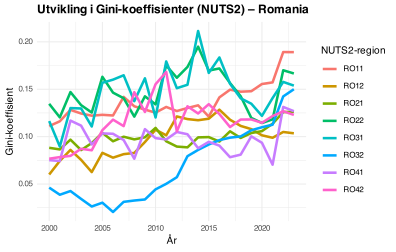
\includegraphics[keepaspectratio]{Assignment1_MSB104_files/figure-pdf/unnamed-chunk-16-1.pdf}}

\begin{verbatim}
<theme> List of 1
 $ plot.title: <ggplot2::element_text>
  ..@ family       : NULL
  ..@ face         : chr "bold"
  ..@ italic       : chr NA
  ..@ fontweight   : num NA
  ..@ fontwidth    : num NA
  ..@ colour       : NULL
  ..@ size         : num 15
  ..@ hjust        : NULL
  ..@ vjust        : NULL
  ..@ angle        : NULL
  ..@ lineheight   : NULL
  ..@ margin       : NULL
  ..@ debug        : NULL
  ..@ inherit.blank: logi FALSE
 @ complete: logi FALSE
 @ validate: logi TRUE
\end{verbatim}

Regionene ITC 4 og ITG2 skiller seg ut her da de gjennom hele rekken har
en koeffisient mellom 0,10 og 0,17. Dette tyder på at i disse regionene
er det en større skjevfordeling av BNPPI enn i resten av landet. I en
gjennomsnittsberegning av den gjennomsnittlige Koeffisienten per år
ligger den på rundt 0,05.

\pandocbounded{\includegraphics[keepaspectratio]{Assignment1_MSB104_files/figure-pdf/unnamed-chunk-17-1.pdf}}

\pandocbounded{\includegraphics[keepaspectratio]{Assignment1_MSB104_files/figure-pdf/unnamed-chunk-18-1.pdf}}

\pandocbounded{\includegraphics[keepaspectratio]{Assignment1_MSB104_files/figure-pdf/unnamed-chunk-19-1.pdf}}

\pandocbounded{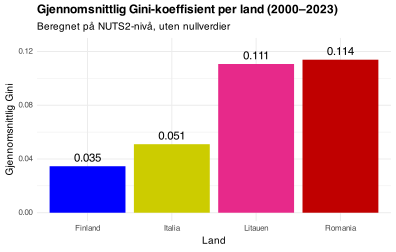
\includegraphics[keepaspectratio]{Assignment1_MSB104_files/figure-pdf/unnamed-chunk-20-1.pdf}}

\begin{longtable}[]{@{}lcccc@{}}
\caption{Gjennomsnittlig Gini-koeffisient per land (uten
0-verdier)}\tabularnewline
\toprule\noalign{}
land & gjennomsnitt\_gini & sd\_gini & min\_gini & max\_gini \\
\midrule\noalign{}
\endfirsthead
\toprule\noalign{}
land & gjennomsnitt\_gini & sd\_gini & min\_gini & max\_gini \\
\midrule\noalign{}
\endhead
\bottomrule\noalign{}
\endlastfoot
Romania & 0.1139 & 0.0350 & 0.0205 & 0.2114 \\
Litauen & 0.1107 & 0.0095 & 0.0920 & 0.1245 \\
Italia & 0.0510 & 0.0364 & 0.0001 & 0.1638 \\
Finland & 0.0346 & 0.0132 & 0.0115 & 0.0643 \\
\end{longtable}

\pandocbounded{\includegraphics[keepaspectratio]{Assignment1_MSB104_files/figure-pdf/unnamed-chunk-22-1.pdf}}

\pandocbounded{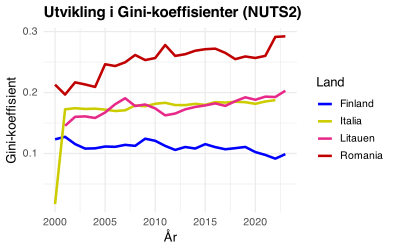
\includegraphics[keepaspectratio]{Assignment1_MSB104_files/figure-pdf/unnamed-chunk-23-1.pdf}}

I tabellen over ser vi GINI koeffisienten for alle NUTS2 regionene som
tilhører vårt datasett. GINI verdien beskriver hvor jevn fordelt BNPPI
er fordelt mellom NUTS3 regionene som havner i samme NUTS2 region.
Koeffisienten ligger i mellom 0,02 og 0,11 for majoriteten av regionene
gjennom hele årrekken. Dette indikerer at i hver enkelt NUTS2 region er
det en jevn fordeling av BNPPI i de tilhørende NUTS3 regionene.

\pandocbounded{\includegraphics[keepaspectratio]{Assignment1_MSB104_files/figure-pdf/unnamed-chunk-24-1.pdf}}

Her er det laget et linediagram som viser utviklingen av GINI koefisient
på NUTS1 region basert på fordelingen av BNPPI i NUTS2 regionene. Dette
tallet sier noe om fordelingen av BNPPI mellom NUTS2 regioner sett opp
mot hele landet. Koefisienten ligger mellom 0,17 og 0,19. Dette
indikerer at det i Italia er en større skjevfordeling mellom NUTS2
regionene, enn det er i NUTS 3 regionene satt opp mot regioner i samme
NUT2.

\subsection{Diskusjon}\label{diskusjon}

De beregnede Gini-koeffisientene for BNP per innbygger på NUTS2-nivå
viser tydelige forskjeller i graden av regional ulikhet mellom landene i
utvalget. Romania og Litauen har de høyeste gjennomsnittlige
Gini-verdiene på henholdsvis 0,1139 og 0,1107, mens Italia (0,0510) og
Finland (0,0346) viser langt lavere nivåer av regional ulikhet. Dette
innebærer at de østeuropeiske landene, som i større grad har vært
gjennom en overgangsøkonomi og rask omstilling etter EU-innlemmelsen,
fortsatt opplever mer betydelige forskjeller i økonomisk utvikling
mellom regionene sammenlignet med de mer etablerte økonomiene i Vest- og
Nord-Europa.

\textbf{Romania} skiller seg ut som landet med størst regional ulikhet.
Både gjennomsnittet og variasjonen (standardavvik = 0.0350) er høye, noe
som indikerer store forskjeller mellom regionene og betydelig endring
over tid.

Resultatene fra analysen viser tydelige mønstre i den regionale
økonomiske ulikheten mellom de fire landene. Italia og Finland, som
begge har modne og diversifiserte økonomier, viser lave og stabile
Gini-koeffisienter. Dette indikerer at at inntektsnivået mellom regionen
er relativt balansert, og at den økonomiske veksten har vært jevnt
fordelt. Italia har likevel små, men medvarende forskjeller mellom nord
og sør, noe som gjenspeiles i at enkelte NUTS2-regioner ligger over
landsgjennomsnittet.

Romania og Litauen viser derimot høyere Gini-koeffisienter, som peker på
større regionale forskjeller. i Romania skyldes dette i stor grad
forskjellen mellom hovedstadregionen Bucuresti-Ilfov og de litt mer
landlige regionene. Litauen viser et lignende mønster, med rask vekst i
Vilnius-regionen sammenlignet med de sørlige og østlige områdene.

Over tid ser vi altså en økende konvergens mellom landene, men fortsatt
betydelig intern ulikhet i de nye EU-medlemmene. Denne utviklingen kan

Gjennomsnittlig BNP per innbygger i utvalget er \textbf{19 883 euro},
med et standardavvik på \textbf{11 386 euro}, noe som viser en tydelig
variasjon i økonomisk velstand mellom regionene. Minimumsverdien er
\textbf{825 euro}, mens maksimum når opp mot \textbf{66 633 euro}, som
reflekterer store forskjeller mellom utviklede regioner i Italia og
Finland sammenlignet med mindre utviklede områder i Romania og Litauen.
Medianverdien på \textbf{20 462 euro} ligger nær gjennomsnittet, noe som
indikerer en tilnærmet symmetrisk fordeling, men noen enkelte regioner
med svært høyt BNP per innbygger trekker gjennomsnittet litt opp.

Over tid viser dataene en jevn vekst i BNP per innbygger i alle fire
land. Finland og Italia hadde de høyeste nivåene gjennom hele perioden,
mens Romania og Litauen viser sterk vekst og gradvis konvergens mot de
rike landene etter 2010. Figurene nedenfor illustrerer både
tidsutviklingen i gjennomsnittlig BNP per innbygger og fordelingen
mellom regionene i det siste observasjonsåret, som danner grunnlaget for
videre analyse av regional ulikhet i del B.




\end{document}
